\documentclass[10pt]{article}
\usepackage[margin=1in, paperwidth=8.5in, paperheight=11in]{geometry}
\usepackage{ifpdf, amsmath, amssymb, comment, color, graphicx, stmaryrd, setspace, enumitem, fancyhdr, wrapfig, textcomp, mathptmx, siunitx, multicol}
\usepackage{hyperref}
\hypersetup{
    colorlinks=true,
    urlcolor=blue,
}

\usepackage{tikz}
\usetikzlibrary{trees}

\setlength{\headheight}{14.5pt}
\newcommand{\del}{\nabla}
\newcommand{\Q}{\mathbb{Q}}
\newcommand{\R}{\mathbb{R}}
\newcommand{\Z}{\mathbb{Z}}
\newcommand{\vu}{\mathbf{u}}
\newcommand{\vv}{\mathbf{v}}
\newcommand{\vw}{\mathbf{w}}
\newcommand{\vi}{\mathbf{i}}
\newcommand{\vj}{\mathbf{j}}
\newcommand{\vk}{\mathbf{k}}
\newcommand{\vn}{\mathbf{n}}
\newcommand{\vr}{\mathbf{r}}
\newcommand{\vs}{\mathbf{s}}
\newcommand{\va}{\mathbf{a}}
\newcommand{\vF}{\mathbf{F}}
\newcommand{\vL}{\mathbf{L}}
\newcommand{\vT}{\mathbf{T}}
\newcommand{\vN}{\mathbf{N}}
\newcommand{\vB}{\mathbf{B}}
\newcommand{\comp}{\operatorname{comp}}
\newcommand{\proj}{\operatorname{proj}}
\newcommand{\orth}{\operatorname{orth}}
\newcommand\dotp[1][.5]{\,\mathbin{\vcenter{\hbox{\scalebox{#1}{$\bullet$}}}}\,}


\newenvironment{red}{\color{red}}{\ignorespacesafterend}
\newcommand{\blue}[1]{\textcolor{blue}{#1}}
\newcommand{\green}[1]{\textcolor{green}{#1}}
\renewcommand{\section}[1]{\begin{center} \textbf{#1} \\\end{center}}
%
\hyphenpenalty=5000
\setlength{\parindent}{0in}
%\oddsidemargin=-.25in
\allowdisplaybreaks
\pagestyle{fancy}
\renewcommand{\headrulewidth}{0pt}
\lhead{MATH 203}
\rhead{Fall 2024}
%\lfoot{}
%\cfoot{}

\begin{document}
%


%\onehalfspacing
\allowdisplaybreaks
%##################################################################
\section{PS\#5 - Arc length, curvature, limits - \red{Answer key} }

\begin{enumerate}[leftmargin=0pt]
    \item Choose your favorite 3D space curve from the Examples menu in CalcPlot3D. Calculate its arc length. Use Wolfram$|$Alpha or similar to calculate the integral numerically because it's probably impossible to find an antiderivative. Look at your space curve and say why the number you got makes sense.
        
    \begin{red}
    I chose Viviani's curve (which, interestingly, is the intersection between a sphere and a cylinder that's tangent to the sphere and goes through the center of the sphere).
    
    The integrand is $|\vr'(t)|$:
    \begin{align*}
        \vr(t) &= \left\langle 1 + \cos t, \sin t, 2 \sin \tfrac{t}{2} \right\rangle \\
        \vr'(t) &= \left\langle -\sin t, \cos t, \cos \tfrac{t}{2} \right\rangle \\
        |\vr'(t)| &= \sqrt{ 
        (-\sin t)^2 + (\cos t)^2 + \left(\cos \tfrac{t}{2}\right)^2
        }\\
        &= \sqrt{\sin^2 t + \cos^2 t + \cos^2\left(\tfrac{t}{2}\right)} \\
        &= \sqrt{1 + \cos^2\left(\tfrac{t}{2}\right)}
    \end{align*}
    (I imagine I could use some trig identities to simplify this further, but I don't ever remember any trig identities besides the Pythagorean identity, lol.)
    
    My bounds of integration should be from $-2\pi$ to $2\pi$, based on the bounds that are programmed into CalcPlot3D. As I look at the ``trace'' arrows moving around the curve, this does indeed appear to produce one full trip around the curve.
    
    So, my integral should be:
    \[ \int_{-2\pi}^{2\pi} \sqrt{1 + \cos^2\left(\tfrac{t}{2}\right)} \, dt \]
    This integrand probably does not have an antiderivative. That means I can't use the fundamental theorem of calculus to compute the definite integral. Darn! I'll just use Wolfram$|$Alpha instead. Fun fact: you can type LaTeX directly into Wolfram$|$Alpha and it will interpret it correctly. Here's my result:
    \begin{center}
        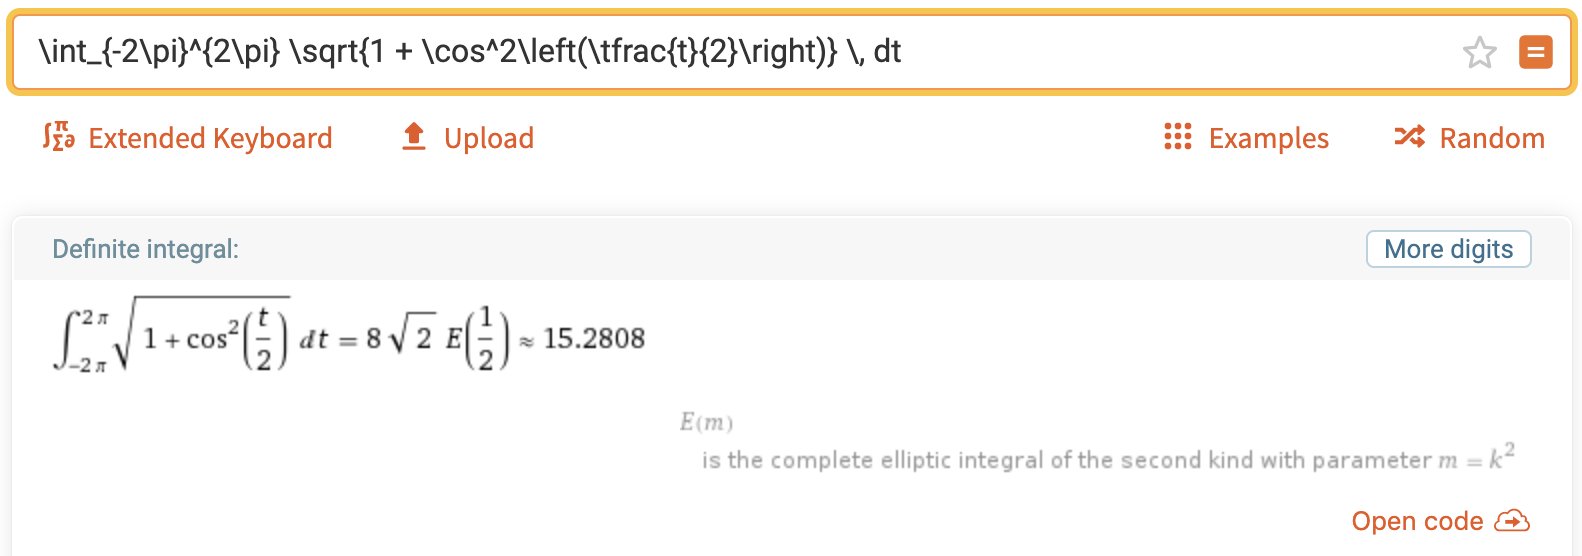
\includegraphics[width=0.75\textwidth]{../images/wa-arc-length.png}
    \end{center}
    This whole business about ``the complete elliptic integral of the second kind'' is W$|$A telling you that there's no elementary antiderivative of this particular integrand. Fortunately, it's smart enough to compute a pretty good numerical approximation, 15.2808.
    
    This value does seem plausible. I think you could reasonably approximate this curve by gluing a couple of circles with radius $\sqrt{2}$ together, and each one of those is going to have circumference $2\cdot\pi\cdot\sqrt{2} \approx 2 \cdot 3 \cdot 1.5 = 9$. So getting something close to 18 is pretty good, I guess.
    \end{red}
    
    \item (AC Multi 10.1 Exercise 15) Use the properties of continuity to determine the set of points at which each of the following functions is continuous. Justify your answers.
    \begin{enumerate}
        \item The function $f$ defined by $f(x,y) = \dfrac{x+2y}{x-y}$
        
        \begin{red}
        This function is continuous everywhere the denominator is nonzero -- that is, whenever $x\neq y$.
        \end{red}
        \item The function $g$ defined by $g(x,y) = \dfrac{\sin(x)}{1+e^y}$
        
        \begin{red}
        The only issue here would be if the denominator was ever zero -- that is, if $1+e^y = 0$. However, since $e^y$ is always positive, $1+e^y$ is never 0, so this function is continuous for all $(x, y)\in \R^2$.
        \end{red}
        \item The function $h$ defined by \begin{equation*}
        h(x,y) = \begin{cases} 
            \dfrac{xy}{x^2+y^2} & \textrm{ if } (x,y) \neq (0,0)  \\ 
            0 & \textrm{ if } (x,y) = (0,0) 
        \end{cases}
        \end{equation*}
        
        \begin{red}
        This function is clearly ok everywhere but $(0,0)$, which is going to require a little more investigation. 
        
        Approaching $(0,0)$ along $y=0$, we see that $h(x,y) = h(x,0) = \dfrac{0}{x^2} = 0$, but approaching $(0, 0)$ along $y=x$, we see that $\displaystyle h(x, y) = h(x,x) = \frac{x^2}{x^2+x^2} = \frac{1}{2} $. Therefore, $\displaystyle\lim_{(x,y)\to(0,0)}h(x,y)$ does not exist, so $h$ is not continuous at $(0,0)$ -- no matter what value we define for $h$ there.
        
        So, overall, $h$ is continuous everywhere except $(0,0)$.
        \end{red}
        \item The function $k$ defined by
        \begin{equation*}
        k(x,y) = \begin{cases} 
            \dfrac{x^2y^4}{x^2+y^2} & \textrm{ if } (x,y) \neq (0,0)  \\ 
            0 & \textrm{ if } (x,y) = (0,0) 
        \end{cases}
        \end{equation*}
        
        \begin{red}
        {\everymath{\displaystyle}
        Again, this function is clearly ok everywhere but $(0,0)$, which is going to require a little more investigation.
        
        By Example 10.1.14, we know that $\lim_{(x,y)\to(0,0)} \frac{x^2y^2}{x^2+y^2} =0.$ Note that $k(x,y) = y^2 \cdot \frac{x^2y^2}{x^2+y^2}$, and that $y^2$ is continuous everywhere. By the properties of limits, 
        \[\lim_{(x,y)\to(0,0)}  \left(y^2 \cdot \frac{x^2y^2}{x^2+y^2}\right) = \left(\lim_{(x,y)\to(0,0)} y^2 \right) \cdot \left(\lim_{(x,y)\to(0,0)} \frac{x^2y^2}{x^2+y^2}\right) = 0 \cdot 0 = 0\] Therefore, since the limit and the value of $k(0,0)$ match, $k$ is indeed continuous at $(0,0)$.
        }
        \end{red}
    \end{enumerate}
    
    \item OPTIONAL FOR A BONUS TOKEN: Let's think about \textbf{the} unit normal vector $\vN(t)$. 
    
    For any space curve $\vr(t)$, you can always find the unit tangent vector $\vT(t)$ by simply ``unitizing'' $\vr'(t)$:
    \[\vT(t) = \frac{\vr'(t)}{|\vr'(t)|}\]
    Explain why $|\vT(t)| = 1$ means that $\vT'(t)$ is orthogonal to $\vT(t)$ at every time $t$.
    
    (Hint: Consider $\vT \dotp \vT$. It might be nice to take the derivative of this, so that $\vT'$ shows up. Use the product rule. But also, note that $\vT \dotp \vT = |\vT|^2 = 1$, which is a constant. What's the derivative of a constant?)
    
    So, if you were going to define \textbf{the} unit normal vector $\vN(t)$, how might you define it? Why does your definition make sense?
    
    \begin{red}
        Following the hint, I'm going to compute $\frac{d}{dt} \left[ \vT \dotp \vT\right]:$
        \begin{align*}
            \frac{d}{dt} \left[ \vT \dotp \vT\right] &= 
            \frac{d}{dt}[\vT] \dotp \vT + \vT \dotp \frac{d}{dt}[\vT]\\
            &= \vT' \dotp \vT + \vT \dotp \vT' \\
            &= 2 (\vT' \dotp \vT)
        \end{align*}
        But on the other hand, since $\vT \dotp \vT = 1$, $\frac{d}{dt} \left[ \vT \dotp \vT\right]$ has to equal 0. Therefore, 
        \[0 = 2 (\vT' \dotp \vT),\]
        so $\vT'$ must be orthogonal to $\vT$. Yay!
        
        So, if I was going to define \textbf{the} unit normal vector $\vN(t)$, I might say $\vN(t) = \dfrac{\vT'(t)}{|\vT'(t)|}$. It's always orthogonal to $\vT(t)$, so it's always normal to the space curve $\vr(t)$.
    \end{red}
    
    {\everymath{\displaystyle}
    \item OPTIONAL FOR A BONUS TOKEN (AC Multi 9.8 Exercise 15) In this exercise we verify the curvature formula \[\kappa = \frac{\lvert \vr'(t) \times \vr''(t) \rvert}{\lvert \vr'(t) \rvert^3}.\]
    \begin{enumerate}
        \item Explain why $\displaystyle \lvert \vr'(t) \rvert = \frac{ds}{dt}.$
        
        \begin{red}
            Let's start by remembering what $s(t)$ is: it's the function that tells us how far we've gone by time $t$, so it's the accumulation function of the speed of the particle:
            \begin{align*}
                 s(t) &= \int_0^t |\vr'(u)|\ du
                 \intertext{Therefore,}
                 \frac{ds}{dt} &= \frac{d}{dt} \left[ \int_0^t |\vr'(u)|\ du\right] = |\vr'(t)|,
            \end{align*}
            by the fundamental theorem of calculus.
        \end{red}
        
        \item Use the fact that $\vT(t) = \frac{\vr'(t)}{\lvert \vr'(t) \rvert}$ and $\lvert \vr'(t) \rvert = \frac{ds}{dt}$ to explain why $\vr'(t) = \frac{ds}{dt} \vT(t)$.
        
        \begin{red}
        Let's start with $\frac{ds}{dt}\cdot \vT(t)$ and just substitute some stuff in.
            \begin{align*}
                \frac{ds}{dt}\cdot \vT(t) &= 
                |\vr'(t)|\cdot \vT(t) =
                |\vr'(t)| \cdot \left(\frac{\vr'(t)}{\lvert \vr'(t) \rvert}\right) = \vr'(t).
            \end{align*}
        \end{red}
        
        \item The Product Rule shows that $\vr''(t) = \frac{d^2s}{dt^2} \vT(t) + \frac{ds}{dt} \vT'(t).$ Explain why $\vr'(t) \times \vr''(t) = \left(\frac{ds}{dt}\right)^2 (\vT(t) \times \vT'(t)).$
        
        \begin{red}
            \begin{align*}
                \vr'(t) \times \vr''(t) &=
                \left[\frac{ds}{dt}\cdot \vT(t)\right]
                \times
                \left[\frac{d^2s}{dt^2} \vT(t) + \frac{ds}{dt} \vT'(t)\right]
                \intertext{$\frac{ds}{dt}$ is a scalar, so we can factor it out of the first term:}
                &= \frac{ds}{dt} \left(
                \left[\vT(t)\right]
                \times
                \left[\frac{d^2s}{dt^2} \vT(t) + \frac{ds}{dt} \vT'(t)\right]
                \right)
                \intertext{We know the cross product distributes:}
                &= \frac{ds}{dt} \left(
                \left[\vT(t) \times \frac{d^2s}{dt^2} \vT(t) \right] +
                \left[\vT(t) \times \frac{ds}{dt} \vT'(t) \right]
                \right)
                \intertext{The first cross product is $\mathbf{0}$, since $\vT(t)$ is certainly parallel to $\frac{d^2s}{dt^2} \vT(t).$ }
                &= \frac{ds}{dt} \left(\vT(t) \times \frac{ds}{dt} \vT'(t) \right)
                \intertext{We can again factor out a $\frac{ds}{dt}$, this time from the second term:}
                &= \left( \frac{ds}{dt} \right)^2 (\vT(t) \times \vT'(t))
            \end{align*}
            Yay, we have arrived at what we wanted.
        \end{red}
        \item In the previous exercise (\#3 on this Problem Set), we explained why $|\vT(t)| = 1$ means that $\vT'(t)$ is orthogonal to $\vT(t)$ at every time $t$. Explain what this tells us about $|\vT(t) \times \vT'(t)|$ and conclude that \[\lvert \vr'(t) \times \vr''(t) \rvert = \left(\frac{ds}{dt}\right)^2 \lvert \vT'(t) \rvert.\]
        
        \begin{red}
            I'm going to use the fact that $|\vu\times\vv| = |\vu||\vv|\sin(\theta)$. In this case, $|\vT(t) \times \vT'(t)| = |\vT(t)| \cdot |\vT'(t)| \cdot \sin(\theta)$, and $\sin(\theta) = 1$ since the two vectors are always orthogonal. Therefore, $|\vT(t) \times \vT'(t)| = |\vT(t)| \cdot |\vT'(t)| = 1 \cdot |\vT'(t)| = |\vT'(t)|$, since $|\vT(t)| =1$.
            Therefore, 
            \begin{align*}
                |\vr'(t) \times \vr''(t)| &=
                \left\lvert \left( \frac{ds}{dt} \right)^2 (\vT(t) \times \vT'(t)) \right \rvert \\
                &= \left( \frac{ds}{dt} \right)^2 \lvert \vT(t) \times \vT'(t) \rvert \\
                &= \left( \frac{ds}{dt} \right)^2 |\vT'(t)|.
            \end{align*}
        \end{red}
        
        \item Finally, use the fact that $\kappa = \frac{\lvert \vT'(t) \rvert }{\lvert \vr'(t) \rvert}$ to verify that $\kappa = \frac{\lvert \vr'(t) \times \vr''(t) \rvert}{\lvert \vr'(t) \rvert^3}.$
        
        \begin{red}
            Since $\lvert \vr'(t) \times \vr''(t) \rvert = \left(\frac{ds}{dt}\right)^2 \lvert \vT'(t) \rvert$, it's certainly true that $|\vT'(t)| = \frac{\lvert \vr'(t) \times \vr''(t) \rvert}{\left(\frac{ds}{dt}\right)^2}$, and since $\frac{ds}{dt} = |\vr'(t)|$, it's certainly true that $\frac{\lvert \vr'(t) \times \vr''(t) \rvert}{\left(\frac{ds}{dt}\right)^2} = \frac{\lvert \vr'(t) \times \vr''(t) \rvert}{|\vr'(t)|^2}$. Therefore,
            \begin{align*}
                \kappa &= \frac{\lvert \vT'(t) \rvert }{\lvert \vr'(t) \rvert} \\
                &= \frac{1}{\lvert \vr'(t) \rvert} \cdot |\vT'(t)| \\
                &=  \frac{1}{\lvert \vr'(t) \rvert} \cdot \frac{\lvert \vr'(t) \times \vr''(t) \rvert}{|\vr'(t)|^2} \\
                &= \frac{\lvert \vr'(t) \times \vr''(t) \rvert}{|\vr'(t)|^3}.
            \end{align*}
            Phew, that was some serious algebra!!
        \end{red}
    \end{enumerate}
    }


    \item For any space curve $\vr(t)$, you can always find the unit tangent vector $\vT(t)$ by simply ``unitizing'' $\vr'(t)$:
    \[\vT(t) = \frac{\vr'(t)}{|\vr'(t)|}\]
    Explain why $|\vT(t)| = 1$ means that $\vT'(t)$ is orthogonal to $\vT(t)$ at every time $t$.
    
    (Hint: Consider $\vT \dotp \vT$. It might be nice to take the derivative of this, so that $\vT'$ shows up. Use the product rule. But also, note that $\vT \dotp \vT = |\vT|^2 = 1$, which is a constant. What's the derivative of a constant?)
    
    So, if you were going to define \textbf{the} unit normal vector $\vN(t)$, how might you define it? Why does your definition make sense?
    
    \begin{red}
        Following the hint, I'm going to compute $\frac{d}{dt} \left[ \vT \dotp \vT\right]:$
        \begin{align*}
            \frac{d}{dt} \left[ \vT \dotp \vT\right] &= 
            \frac{d}{dt}[\vT] \dotp \vT + \vT \dotp \frac{d}{dt}[\vT]\\
            &= \vT' \dotp \vT + \vT \dotp \vT' \\
            &= 2 (\vT' \dotp \vT)
        \end{align*}
        But on the other hand, since $\vT \dotp \vT = 1$, $\frac{d}{dt} \left[ \vT \dotp \vT\right]$ has to equal 0. Therefore, 
        \[0 = 2 (\vT' \dotp \vT),\]
        so $\vT'$ must be orthogonal to $\vT$. Yay!
        
        So, if I was going to define \textbf{the} unit normal vector $\vN(t)$, I might say $\vN(t) = \dfrac{\vT'(t)}{|\vT'(t)|}$. It's always orthogonal to $\vT(t)$, so it's always normal to the space curve $\vr(t)$.
    \end{red}
    
    \item For each of the following prompts, provide an example of a function of two variables with the desired properties (with justification), or explain why such a function does not exist.
    \begin{enumerate}
        \item A function $p$ that is defined at $(0, 0)$, but $\lim_{(x, y) \to (0, 0)} p(x, y)$ does not exist.
        
        \begin{red}
            How about we just take the example in Preview Activity 2.1.1, and define it a value at $(0, 0)$?
            \[ p(x,y) = 
            \begin{cases}
                \frac{2xy}{x^2+y^2}, & (x, y) \neq (0, 0) \\
                17, & (x, y) = (0, 0)
            \end{cases}
            \]
            (Nothing special about the number 17. I just kinda picked it out of thin air.)
            
            Preview Activity 2.1.1 explains why the limit doesn't exist.
        \end{red}
        \item A function $q$ that does not have a limit at $(0, 0)$, but that has the same limiting value along any line $y=mx$ as $x \to 0$. 
        
        \begin{red}
            Webwork 2.1 \#2 will be helpful here:
            \[q(x,y) = \frac{x^{5}y}{x^{10}+y^{5}}\]
            If we approach along $y = mx$, we're looking at $q(x, mx):$
            \begin{align*}
                q(x, mx) &= \frac{x^{5}\cdot (mx)}{x^{10}+(mx)^{5}}
                = \frac{mx^6}{x^{10} + m^5 x^5} \\
                &= \frac{mx^6}{x^5\cdot(x^5+m^5)} 
                = \frac{mx}{x^5+m^5}
            \end{align*}
            So now we can let $x$ go to 0 without anything bad happening:
            \[\lim_{x\to 0} q(x, mx) = \lim_{x \to 0} \frac{mx}{x^5+m^5} = \frac{m\cdot 0}{0^5 + m^5} = 0,\]
            no matter what the value of $m$.
            
            However, something different will happen if we approach $(0, 0)$ along $y=x^5$:
            \begin{align*}
                q(x, x^5) &= \frac{x^{5}\cdot (x^5)}{x^{10}+(x^5)^{5}}
                = \frac{x^{10}}{x^{10} + x^{25}} \\
                &= \frac{x^{10}}{x^{10}\cdot(1 + x^{15})} 
                = \frac{1}{1 + x^{15}}.
            \end{align*}
            Again, we can now let $x$ go to 0 without anything bad happening, but we get something different:
            \[\lim_{x\to 0} q(x, x^5) = \lim_{x\to 0}\frac{1}{1 + x^{15}} = \frac{1}{1+0} = 1.\]
            Therefore, the limit doesn't exist, because we've found two paths that give us different limiting values.
        \end{red}
        
        \item A function $r$ that is continuous at $(0, 0)$, but $\lim_{(x, y) \to (0, 0)} r(x, y)$ does not exist.
        
        \begin{red}
            This one's not gonna work. If $r$ is continuous at $(0, 0)$, the limit \textbf{must} exist -- and must in fact be the same value as the function value $r(0,0)$.
        \end{red}
        
        \item A function $s$ such that 
        \[\lim_{(x, x) \to (0, 0)} s(x, x) = 3 \quad \textrm{and} \quad
        \lim_{(x, 2x) \to (0, 0)} s(x, 2x) = 6,\]
        for which $\lim_{(x, x) \to (0, 0)} s(x, y)$ exists.
        
        \begin{red}
            This one's not gonna work either. We've shown that there's two directions along which we can approach $(0, 0)$ that give us two different limiting values: along $y=x$, the limiting value is 3, but along $y=2x$, the limiting value is 6. Since there's two directions with two different limiting values, the overall limit can't exist.
        \end{red}
        
        \item A function $t$ that is not defined at $(1, 1)$, but $\lim_{(x, x) \to (1, 1)} t(x, y)$ does exist.
        
        \begin{red}
            One such function:
            \[t(x, y) = \frac{(x^2-1)(y^2-1)}{(x-1)(y-1)}\]
            Note that the numerator factors as $(x-1)(x+1)(y-1)(y+1)$. As long as $x\neq 1$, the $(x-1)$s that appear in the numerator and denominator can divide to 1. (This won't work when $x=1$, because $0/0$ is indeterminate.) When I'm taking the limit as $x$ \textbf{approaches} 1, $x$ doesn't \textbf{equal} 1 -- so we can divide that problematic term out. The same logic applies to the $y$ terms -- the overall value of the limit is 4.
            
            (Note that this is the same logic by which the limit definition of the derivative works.)
        \end{red}
    
    \end{enumerate}

\end{enumerate}

\begin{red}
\textbf{Learning Targets Reflection:} V1, V2, maybe S1, D2, D5. Maybe some others.
\end{red}

\end{document}